\documentclass{whiteboard}
\begin{document}
\begin{frame}[plain,t]
\bbcover{OBI 2013 - Nível Júnior: Fase 1}{Capital}{Prof. Edson Alves}{Faculdade UnB Gama}

\end{frame}
\begin{frame}[plain,t]
\vspace*{\fill}

\bbtext{O governo do estado de Queensland está com problemas sérios de trânsito na capital Brisbane, onde estão
os prédios administrativos. Para desafogar o trânsito, o prefeito de Brisbane e o governador de Queensland
decidiram que uma nova capital administrativa deve ser construída em uma área fora de Brisbane. Para
projetar a nova capital, o renomado arquiteto minimalista Joe Bloggs foi contratado.}

\vspace{0.2in}

\bbtext{Bloggs foi informado de que o terreno destinado à nova capital ainda não foi demarcado, mas será retangular.
Além disso, a cidade deverá ser dividida em quatro zonas, uma delas destinada a uma reserva ambiental
e cada uma das outras três receberá os novos prédios de cada um dos três poderes (Executivo, Legislativo
e Judiciário). Em um arroubo de criatividade, Bloggs decidiu que duas avenidas, perpendiculares entre si,
cada uma paralela a dois dos lados do terreno retangular, dividirão a capital nas quatro zonas.}

\vspace*{\fill}
\end{frame}
\begin{frame}[plain,t]
\vspace*{\fill}

\bbtext{Bloggs recebeu do governo as áreas de cada uma das zonas e, após muito esforço, encontrou um retângulo que
pode ser dividido conforme seus planos e de forma a respeitar as áreas delimitadas. No entanto, a Fundação
de Conservação dos Cangurus determinou que a área destinada à reserva ambiental era muito pequena, o
que obrigou o governo a alterar as áreas das quatro zonas. Após receber as novas medidas, Bloggs tentou
encontrar um novo retângulo que viabilizasse seu projeto, porém sem sucesso. Cansado de fazer testes,
ele pensou que talvez tenha que abandonar sua brilhante ideia. Por isso, ele pediu para você escrever um
programa que, dadas as áreas das quatro zonas, determine se ele poderá ou não manter seu projeto (ou seja,
se existe um retângulo que possa ser dividido por duas retas perpendiculares, cada uma paralela a dois dos
lados do retângulo, tal que as quatro áreas formadas obedeçam às exigências do governo).}

\vspace*{\fill}
\end{frame}
\begin{frame}[plain,t]
\vspace*{\fill}

\bbbold{Entrada}

\vspace{0.2in}

\bbtext{A entrada consiste de uma única linha contendo quatro inteiros $A_1$, $A_2$, $A_3$, $A_4$, indicando a área de cada
uma das zonas.}

\vspace{0.2in}

\bbbold{Saída}

\vspace{0.2in}

\bbtext{Imprima uma única linha contendo um único caractere: `\texttt{S}' se Bloggs pode preservar seu projeto e `\texttt{N}' caso
contrário.}

\vspace{0.2in}

\bbbold{Restrições}
\vspace{-0.1in}

\bbtext{
\begin{itemize}
\item $1 \leq A_i \leq 10^4$
\end{itemize}
}

\vspace*{\fill}
\end{frame}
\begin{frame}[plain,t]
\begin{tikzpicture}
\node[draw,opacity=0] at (0, 0) {x};
\node[draw,opacity=0] at (14, 8) {x};

	\node[anchor=west] (header) at (0, 7.0) { \bbbold{Exemplo de entrada e saída} };

\end{tikzpicture}
\end{frame}
\begin{frame}[plain,t]
\begin{tikzpicture}
\node[draw,opacity=0] at (0, 0) {x};
\node[draw,opacity=0] at (14, 8) {x};

	\node[anchor=west] (header) at (0, 7.0) { \bbbold{Exemplo de entrada e saída} };


	\node[anchor=west] (line1) at (1.0, 6.0) { \bbtext{\texttt{1 2 4 8}} };

\end{tikzpicture}
\end{frame}
\begin{frame}[plain,t]
\begin{tikzpicture}
\node[draw,opacity=0] at (0, 0) {x};
\node[draw,opacity=0] at (14, 8) {x};

	\node[anchor=west] (header) at (0, 7.0) { \bbbold{Exemplo de entrada e saída} };


	\node[anchor=west] (line1) at (1.0, 6.0) { \bbtext{\texttt{1 2 4 8}} };


	\draw[->,color=BBViolet] (1.25, 5.0) to  (1.25, 5.75);

	\node[] (r) at (1.25, 4.75) { \footnotesize \bbcomment{$A_1$} };

\end{tikzpicture}
\end{frame}
\begin{frame}[plain,t]
\begin{tikzpicture}
\node[draw,opacity=0] at (0, 0) {x};
\node[draw,opacity=0] at (14, 8) {x};

	\node[anchor=west] (header) at (0, 7.0) { \bbbold{Exemplo de entrada e saída} };


	\node[anchor=west] (line1) at (1.0, 6.0) { \bbtext{\texttt{1 2 4 8}} };


	\draw[->,color=BBViolet] (1.625, 5.0) to  (1.625, 5.75);

	\node[] (r) at (1.625, 4.75) { \footnotesize \bbcomment{$A_2$} };



\end{tikzpicture}
\end{frame}
\begin{frame}[plain,t]
\begin{tikzpicture}
\node[draw,opacity=0] at (0, 0) {x};
\node[draw,opacity=0] at (14, 8) {x};

	\node[anchor=west] (header) at (0, 7.0) { \bbbold{Exemplo de entrada e saída} };


	\node[anchor=west] (line1) at (1.0, 6.0) { \bbtext{\texttt{1 2 4 8}} };


	\draw[->,color=BBViolet] (2.025, 5.0) to  (2.025, 5.75);

	\node[] (r) at (2.05, 4.75) { \footnotesize \bbcomment{$A_3$} };





\end{tikzpicture}
\end{frame}
\begin{frame}[plain,t]
\begin{tikzpicture}
\node[draw,opacity=0] at (0, 0) {x};
\node[draw,opacity=0] at (14, 8) {x};

	\node[anchor=west] (header) at (0, 7.0) { \bbbold{Exemplo de entrada e saída} };


	\node[anchor=west] (line1) at (1.0, 6.0) { \bbtext{\texttt{1 2 4 8}} };


	\draw[->,color=BBViolet] (2.425, 5.0) to  (2.425, 5.75);

	\node[] (r) at (2.45, 4.75) { \footnotesize \bbcomment{$A_4$} };













\end{tikzpicture}
\end{frame}
\begin{frame}[plain,t]
\begin{tikzpicture}
\node[draw,opacity=0] at (0, 0) {x};
\node[draw,opacity=0] at (14, 8) {x};

	\node[anchor=west] (header) at (0, 7.0) { \bbbold{Exemplo de entrada e saída} };


	\node[anchor=west] (line1) at (1.0, 6.0) { \bbtext{\texttt{1 2 4 8}} };

















	\draw[very thick] (6, 2) rectangle (11, 5);

\end{tikzpicture}
\end{frame}
\begin{frame}[plain,t]
\begin{tikzpicture}
\node[draw,opacity=0] at (0, 0) {x};
\node[draw,opacity=0] at (14, 8) {x};

	\node[anchor=west] (header) at (0, 7.0) { \bbbold{Exemplo de entrada e saída} };


	\node[anchor=west] (line1) at (1.0, 6.0) { \bbtext{\texttt{1 2 4 8}} };

















	\draw[very thick] (6, 2) rectangle (11, 5);


	\draw[color=gray,thick,dashed] (7, 2) to (7, 5);

	\node[] (b1) at (6.5, 1.65) { $1$ };

	\node[] (b2) at (9.0, 1.65) { $4$ };

\end{tikzpicture}
\end{frame}
\begin{frame}[plain,t]
\begin{tikzpicture}
\node[draw,opacity=0] at (0, 0) {x};
\node[draw,opacity=0] at (14, 8) {x};

	\node[anchor=west] (header) at (0, 7.0) { \bbbold{Exemplo de entrada e saída} };


	\node[anchor=west] (line1) at (1.0, 6.0) { \bbtext{\texttt{1 2 4 8}} };

















	\draw[very thick] (6, 2) rectangle (11, 5);


	\draw[color=gray,thick,dashed] (7, 2) to (7, 5);

	\node[] (b1) at (6.5, 1.65) { $1$ };

	\node[] (b2) at (9.0, 1.65) { $4$ };


	\draw[color=gray,thick,dashed] (6, 3) to (11, 3);

	\node[] (h1) at (5.65, 2.5) { $1$ };

	\node[] (h2) at (5.65, 4.0) { $2$ };

\end{tikzpicture}
\end{frame}
\begin{frame}[plain,t]
\begin{tikzpicture}
\node[draw,opacity=0] at (0, 0) {x};
\node[draw,opacity=0] at (14, 8) {x};

	\node[anchor=west] (header) at (0, 7.0) { \bbbold{Exemplo de entrada e saída} };


	\node[anchor=west] (line1) at (1.0, 6.0) { \bbtext{\texttt{1 2 4 8}} };











	\draw[color=cyan!40,fill=cyan!40] (6, 2) rectangle (7, 3);






	\draw[very thick] (6, 2) rectangle (11, 5);


	\draw[color=gray,thick,dashed] (7, 2) to (7, 5);

	\node[] (b1) at (6.5, 1.65) { $1$ };

	\node[] (b2) at (9.0, 1.65) { $4$ };


	\draw[color=gray,thick,dashed] (6, 3) to (11, 3);

	\node[] (h1) at (5.65, 2.5) { $1$ };

	\node[] (h2) at (5.65, 4.0) { $2$ };


	\node[] (a1_label) at (6.5, 2.5) { $A_1$ };
\end{tikzpicture}
\end{frame}
\begin{frame}[plain,t]
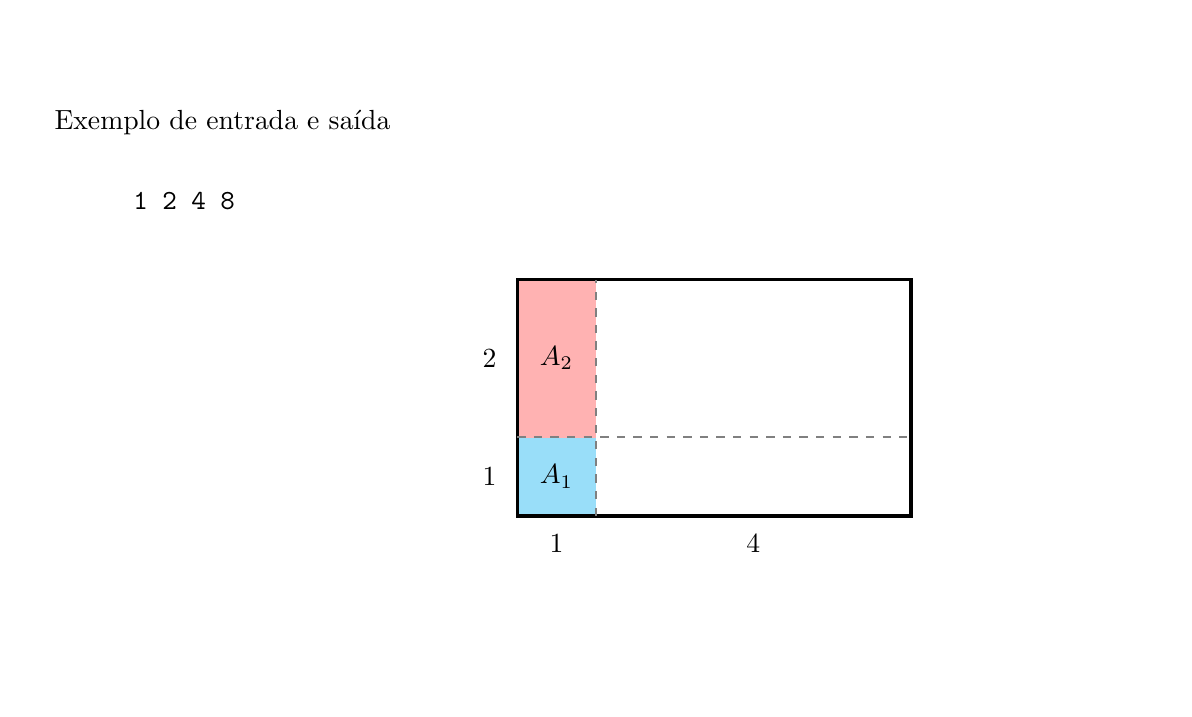
\begin{tikzpicture}
\node[draw,opacity=0] at (0, 0) {x};
\node[draw,opacity=0] at (14, 8) {x};

	\node[anchor=west] (header) at (0, 7.0) { \bbbold{Exemplo de entrada e saída} };


	\node[anchor=west] (line1) at (1.0, 6.0) { \bbtext{\texttt{1 2 4 8}} };











	\draw[color=cyan!40,fill=cyan!40] (6, 2) rectangle (7, 3);


	\draw[color=red!30,fill=red!30] (6, 3) rectangle (7, 5);




	\draw[very thick] (6, 2) rectangle (11, 5);


	\draw[color=gray,thick,dashed] (7, 2) to (7, 5);

	\node[] (b1) at (6.5, 1.65) { $1$ };

	\node[] (b2) at (9.0, 1.65) { $4$ };


	\draw[color=gray,thick,dashed] (6, 3) to (11, 3);

	\node[] (h1) at (5.65, 2.5) { $1$ };

	\node[] (h2) at (5.65, 4.0) { $2$ };


	\node[] (a1_label) at (6.5, 2.5) { $A_1$ };

	\node[] (a2_label) at (6.5, 4.0) { $A_2$ };

\end{tikzpicture}
\end{frame}
\begin{frame}[plain,t]
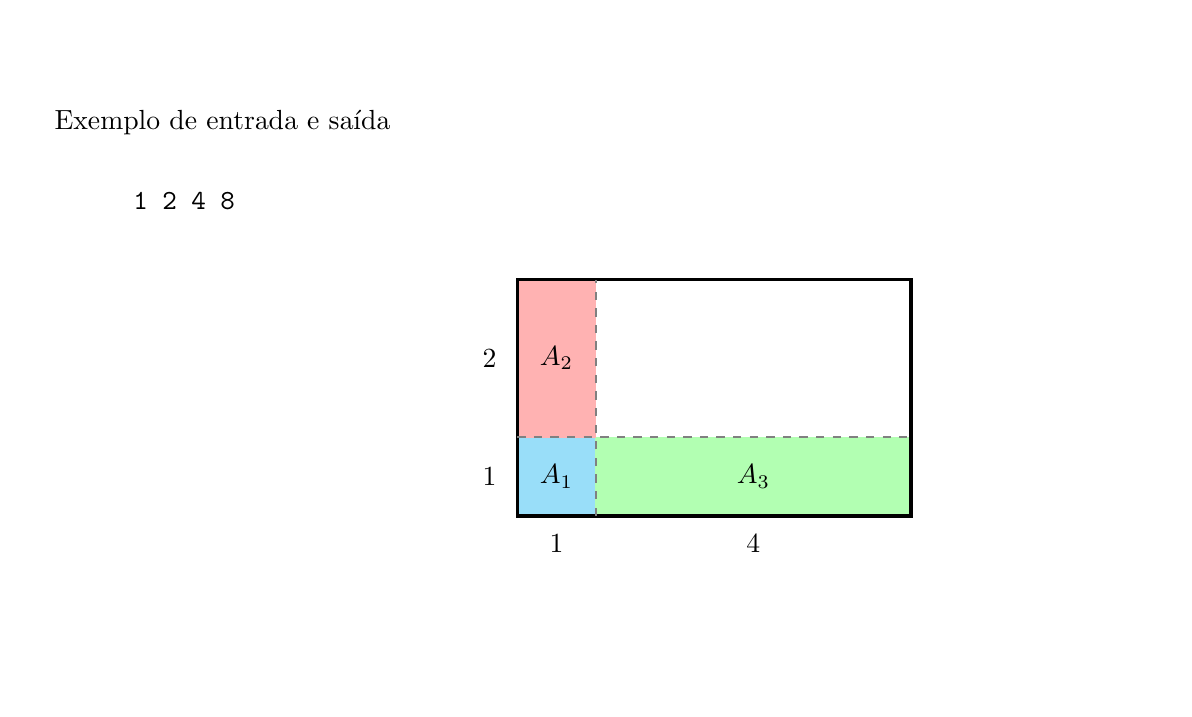
\begin{tikzpicture}
\node[draw,opacity=0] at (0, 0) {x};
\node[draw,opacity=0] at (14, 8) {x};

	\node[anchor=west] (header) at (0, 7.0) { \bbbold{Exemplo de entrada e saída} };


	\node[anchor=west] (line1) at (1.0, 6.0) { \bbtext{\texttt{1 2 4 8}} };











	\draw[color=cyan!40,fill=cyan!40] (6, 2) rectangle (7, 3);

	\draw[color=green!30,fill=green!30] (7, 2) rectangle (11, 3);

	\draw[color=red!30,fill=red!30] (6, 3) rectangle (7, 5);




	\draw[very thick] (6, 2) rectangle (11, 5);


	\draw[color=gray,thick,dashed] (7, 2) to (7, 5);

	\node[] (b1) at (6.5, 1.65) { $1$ };

	\node[] (b2) at (9.0, 1.65) { $4$ };


	\draw[color=gray,thick,dashed] (6, 3) to (11, 3);

	\node[] (h1) at (5.65, 2.5) { $1$ };

	\node[] (h2) at (5.65, 4.0) { $2$ };


	\node[] (a1_label) at (6.5, 2.5) { $A_1$ };

	\node[] (a2_label) at (6.5, 4.0) { $A_2$ };


	\node[] (a3_label) at (9.0, 2.5) { $A_3$ };

\end{tikzpicture}
\end{frame}
\begin{frame}[plain,t]
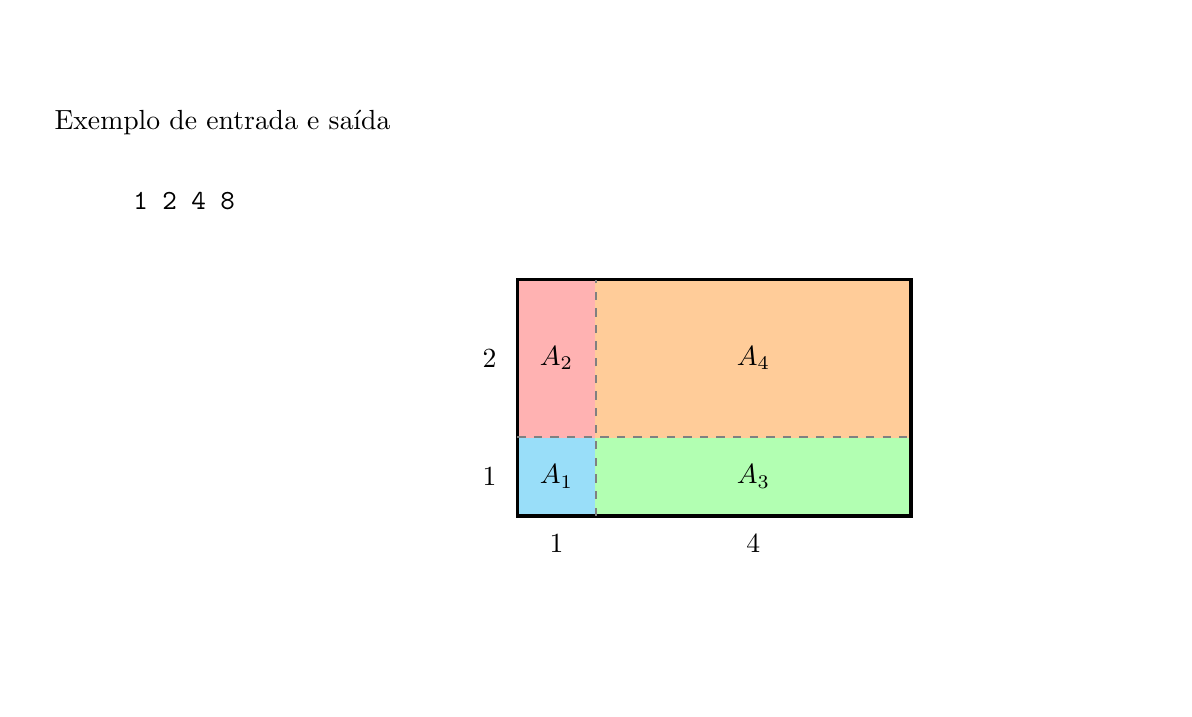
\begin{tikzpicture}
\node[draw,opacity=0] at (0, 0) {x};
\node[draw,opacity=0] at (14, 8) {x};

	\node[anchor=west] (header) at (0, 7.0) { \bbbold{Exemplo de entrada e saída} };


	\node[anchor=west] (line1) at (1.0, 6.0) { \bbtext{\texttt{1 2 4 8}} };











	\draw[color=cyan!40,fill=cyan!40] (6, 2) rectangle (7, 3);

	\draw[color=green!30,fill=green!30] (7, 2) rectangle (11, 3);

	\draw[color=red!30,fill=red!30] (6, 3) rectangle (7, 5);

	\draw[color=orange!40,fill=orange!40] (7, 3) rectangle (11, 5);



	\draw[very thick] (6, 2) rectangle (11, 5);


	\draw[color=gray,thick,dashed] (7, 2) to (7, 5);

	\node[] (b1) at (6.5, 1.65) { $1$ };

	\node[] (b2) at (9.0, 1.65) { $4$ };


	\draw[color=gray,thick,dashed] (6, 3) to (11, 3);

	\node[] (h1) at (5.65, 2.5) { $1$ };

	\node[] (h2) at (5.65, 4.0) { $2$ };


	\node[] (a1_label) at (6.5, 2.5) { $A_1$ };

	\node[] (a2_label) at (6.5, 4.0) { $A_2$ };


	\node[] (a3_label) at (9.0, 2.5) { $A_3$ };


	\node[] (a4_label) at (9.0, 4.0) { $A_4$ };

\end{tikzpicture}
\end{frame}
\begin{frame}[plain,t]
\begin{tikzpicture}
\node[draw,opacity=0] at (0, 0) {x};
\node[draw,opacity=0] at (14, 8) {x};

	\node[anchor=west] (header) at (0, 7.0) { \bbbold{Exemplo de entrada e saída} };


	\node[anchor=west] (line1) at (1.0, 6.0) { \bbtext{\texttt{1 2 4 8}} };


	\draw[->,color=BBViolet] (2.75, 6.0) to  (3.75, 6.0);

	\node[] (r) at (4.0, 6.0) { \footnotesize \bboutput{S} };








	\draw[color=cyan!40,fill=cyan!40] (6, 2) rectangle (7, 3);

	\draw[color=green!30,fill=green!30] (7, 2) rectangle (11, 3);

	\draw[color=red!30,fill=red!30] (6, 3) rectangle (7, 5);

	\draw[color=orange!40,fill=orange!40] (7, 3) rectangle (11, 5);



	\draw[very thick] (6, 2) rectangle (11, 5);


	\draw[color=gray,thick,dashed] (7, 2) to (7, 5);

	\node[] (b1) at (6.5, 1.65) { $1$ };

	\node[] (b2) at (9.0, 1.65) { $4$ };


	\draw[color=gray,thick,dashed] (6, 3) to (11, 3);

	\node[] (h1) at (5.65, 2.5) { $1$ };

	\node[] (h2) at (5.65, 4.0) { $2$ };


	\node[] (a1_label) at (6.5, 2.5) { $A_1$ };

	\node[] (a2_label) at (6.5, 4.0) { $A_2$ };


	\node[] (a3_label) at (9.0, 2.5) { $A_3$ };


	\node[] (a4_label) at (9.0, 4.0) { $A_4$ };






\end{tikzpicture}
\end{frame}
\begin{frame}[plain,t]
\begin{tikzpicture}
\node[draw,opacity=0] at (0, 0) {x};
\node[draw,opacity=0] at (14, 8) {x};

	\node[anchor=west] (title) at (0.0, 7.0) { \Large \bbbold{Solução} };

\end{tikzpicture}
\end{frame}
\begin{frame}[plain,t]
\begin{tikzpicture}
\node[draw,opacity=0] at (0, 0) {x};
\node[draw,opacity=0] at (14, 8) {x};

	\node[anchor=west] (title) at (0.0, 7.0) { \Large \bbbold{Solução} };


	\node[anchor=west] (a) at (1.0, 6.0) { \bbtext{Considere que exista um retângulo de base $b$ e altura $h$} };

\end{tikzpicture}
\end{frame}
\begin{frame}[plain,t]
\begin{tikzpicture}
\node[draw,opacity=0] at (0, 0) {x};
\node[draw,opacity=0] at (14, 8) {x};

	\node[anchor=west] (title) at (0.0, 7.0) { \Large \bbbold{Solução} };


	\node[anchor=west] (a) at (1.0, 6.0) { \bbtext{Considere que exista um retângulo de base $b$ e altura $h$} };


	\draw[very thick] (1, 1) rectangle (9, 5);

	\node[] (b) at (5.0, 0.6) { $b$ };

	\node[] (h) at (0.65, 3.0) { $h$ };

\end{tikzpicture}
\end{frame}
\begin{frame}[plain,t]
\begin{tikzpicture}
\node[draw,opacity=0] at (0, 0) {x};
\node[draw,opacity=0] at (14, 8) {x};

	\node[anchor=west] (title) at (0.0, 7.0) { \Large \bbbold{Solução} };


	\node[anchor=west] (a) at (1.0, 6.0) { \bbtext{Façamos um corte paralelo à altura, dividindo o retângulo em duas partes} };


	\draw[very thick] (1, 1) rectangle (9, 5);

	\node[] (b) at (5.0, 0.6) { $b$ };

	\node[] (h) at (0.65, 3.0) { $h$ };

\end{tikzpicture}
\end{frame}
\begin{frame}[plain,t]
\begin{tikzpicture}
\node[draw,opacity=0] at (0, 0) {x};
\node[draw,opacity=0] at (14, 8) {x};

	\node[anchor=west] (title) at (0.0, 7.0) { \Large \bbbold{Solução} };


	\node[anchor=west] (a) at (1.0, 6.0) { \bbtext{Façamos um corte paralelo à altura, dividindo o retângulo em duas partes} };


	\draw[very thick] (1, 1) rectangle (9, 5);

	\node[] (b) at (2.5, 0.6) { $b_1$ };

	\node[] (h) at (0.65, 3.0) { $h$ };


	\draw[color=gray,dashed] (4, 1) to (4, 5);


	\node[] (b2) at (6.5, 0.6) { $b_2$ };

\end{tikzpicture}
\end{frame}
\begin{frame}[plain,t]
\begin{tikzpicture}
\node[draw,opacity=0] at (0, 0) {x};
\node[draw,opacity=0] at (14, 8) {x};

	\node[anchor=west] (title) at (0.0, 7.0) { \Large \bbbold{Solução} };


	\node[anchor=west] (a) at (1.0, 6.0) { \bbtext{Um novo corte, paralelo à base, divide o retângulo em quatro partes} };


	\draw[very thick] (1, 1) rectangle (9, 5);

	\node[] (b) at (2.5, 0.6) { $b_1$ };

	\node[] (h) at (0.65, 3.0) { $h$ };


	\draw[color=gray,dashed] (4, 1) to (4, 5);


	\node[] (b2) at (6.5, 0.6) { $b_2$ };


\end{tikzpicture}
\end{frame}
\begin{frame}[plain,t]
\begin{tikzpicture}
\node[draw,opacity=0] at (0, 0) {x};
\node[draw,opacity=0] at (14, 8) {x};

	\node[anchor=west] (title) at (0.0, 7.0) { \Large \bbbold{Solução} };


	\node[anchor=west] (a) at (1.0, 6.0) { \bbtext{Um novo corte, paralelo à base, divide o retângulo em quatro partes} };


	\draw[very thick] (1, 1) rectangle (9, 5);

	\node[] (b) at (2.5, 0.6) { $b_1$ };

	\node[] (h) at (0.65, 2.0) { $h_1$ };


	\draw[color=gray,dashed] (4, 1) to (4, 5);


	\node[] (b2) at (6.5, 0.6) { $b_2$ };



	\draw[color=gray,dashed] (1, 3) to (9, 3);


	\node[] (h2) at (0.65, 4.0) { $h_2$ };

\end{tikzpicture}
\end{frame}
\begin{frame}[plain,t]
\begin{tikzpicture}
\node[draw,opacity=0] at (0, 0) {x};
\node[draw,opacity=0] at (14, 8) {x};

	\node[anchor=west] (title) at (0.0, 7.0) { \Large \bbbold{Solução} };


	\node[anchor=west] (a) at (1.0, 6.0) { \bbtext{Suponha que esta divisão tenha gerado partes com áreas $A_1, A_2, A_3$ e $A_4$} };


	\draw[very thick] (1, 1) rectangle (9, 5);

	\node[] (b) at (2.5, 0.6) { $b_1$ };

	\node[] (h) at (0.65, 2.0) { $h_1$ };


	\draw[color=gray,dashed] (4, 1) to (4, 5);


	\node[] (b2) at (6.5, 0.6) { $b_2$ };



	\draw[color=gray,dashed] (1, 3) to (9, 3);


	\node[] (h2) at (0.65, 4.0) { $h_2$ };


\end{tikzpicture}
\end{frame}
\begin{frame}[plain,t]
\begin{tikzpicture}
\node[draw,opacity=0] at (0, 0) {x};
\node[draw,opacity=0] at (14, 8) {x};

	\node[anchor=west] (title) at (0.0, 7.0) { \Large \bbbold{Solução} };


	\node[anchor=west] (a) at (1.0, 6.0) { \bbtext{Suponha que esta divisão tenha gerado partes com áreas $A_1, A_2, A_3$ e $A_4$} };


	\draw[very thick] (1, 1) rectangle (9, 5);

	\node[] (b) at (2.5, 0.6) { $b_1$ };

	\node[] (h) at (0.65, 2.0) { $h_1$ };


	\draw[color=gray,dashed] (4, 1) to (4, 5);


	\node[] (b2) at (6.5, 0.6) { $b_2$ };



	\draw[color=gray,dashed] (1, 3) to (9, 3);


	\node[] (h2) at (0.65, 4.0) { $h_2$ };



	\node[] (a1) at (2.5, 2.0) { $A_1$ };

	\node[] (a2) at (6.5, 2.0) { $A_2$ };

	\node[] (a3) at (2.5, 4.0) { $A_3$ };

	\node[] (a4) at (6.5, 4.0) { $A_4$ };

\end{tikzpicture}
\end{frame}
\begin{frame}[plain,t]
\begin{tikzpicture}
\node[draw,opacity=0] at (0, 0) {x};
\node[draw,opacity=0] at (14, 8) {x};

	\node[anchor=west] (title) at (0.0, 7.0) { \Large \bbbold{Solução} };


	\node[anchor=west] (a) at (1.0, 6.0) { \bbtext{Em relação às áreas $A_1$ e $A_2$, observe que} };


	\draw[very thick] (1, 1) rectangle (9, 5);

	\node[] (b) at (2.5, 0.6) { $b_1$ };

	\node[] (h) at (0.65, 2.0) { $h_1$ };


	\draw[color=gray,dashed] (4, 1) to (4, 5);


	\node[] (b2) at (6.5, 0.6) { $b_2$ };



	\draw[color=gray,dashed] (1, 3) to (9, 3);


	\node[] (h2) at (0.65, 4.0) { $h_2$ };



	\node[] (a1) at (2.5, 2.0) { $A_1$ };

	\node[] (a2) at (6.5, 2.0) { $A_2$ };

	\node[] (a3) at (2.5, 4.0) { $A_3$ };

	\node[] (a4) at (6.5, 4.0) { $A_4$ };


\end{tikzpicture}
\end{frame}
\begin{frame}[plain,t]
\begin{tikzpicture}
\node[draw,opacity=0] at (0, 0) {x};
\node[draw,opacity=0] at (14, 8) {x};

	\node[anchor=west] (title) at (0.0, 7.0) { \Large \bbbold{Solução} };


	\node[anchor=west] (a) at (1.0, 6.0) { \bbtext{Em relação às áreas $A_1$ e $A_2$, observe que} };


	\draw[very thick] (1, 1) rectangle (9, 5);

	\node[] (b) at (2.5, 0.6) { $b_1$ };

	\node[] (h) at (0.65, 2.0) { $h_1$ };


	\draw[color=gray,dashed] (4, 1) to (4, 5);


	\node[] (b2) at (6.5, 0.6) { $b_2$ };



	\draw[color=gray,dashed] (1, 3) to (9, 3);


	\node[] (h2) at (0.65, 4.0) { $h_2$ };



	\node[] (a1) at (2.5, 2.0) { $A_1$ };

	\node[] (a2) at (6.5, 2.0) { $A_2$ };

	\node[] (a3) at (2.5, 4.0) { $A_3$ };

	\node[] (a4) at (6.5, 4.0) { $A_4$ };



	\node[anchor=west] (eq1) at (10.0, 5.0) { $A_1 = b_1h_1$ };

\end{tikzpicture}
\end{frame}
\begin{frame}[plain,t]
\begin{tikzpicture}
\node[draw,opacity=0] at (0, 0) {x};
\node[draw,opacity=0] at (14, 8) {x};

	\node[anchor=west] (title) at (0.0, 7.0) { \Large \bbbold{Solução} };


	\node[anchor=west] (a) at (1.0, 6.0) { \bbtext{Em relação às áreas $A_1$ e $A_2$, observe que} };


	\draw[very thick] (1, 1) rectangle (9, 5);

	\node[] (b) at (2.5, 0.6) { $b_1$ };

	\node[] (h) at (0.65, 2.0) { $h_1$ };


	\draw[color=gray,dashed] (4, 1) to (4, 5);


	\node[] (b2) at (6.5, 0.6) { $b_2$ };



	\draw[color=gray,dashed] (1, 3) to (9, 3);


	\node[] (h2) at (0.65, 4.0) { $h_2$ };



	\node[] (a1) at (2.5, 2.0) { $A_1$ };

	\node[] (a2) at (6.5, 2.0) { $A_2$ };

	\node[] (a3) at (2.5, 4.0) { $A_3$ };

	\node[] (a4) at (6.5, 4.0) { $A_4$ };



	\node[anchor=west] (eq1) at (10.0, 5.0) { $A_1 = b_1h_1$ };


	\node[anchor=west] (eq2) at (10.0, 4.25) { $A_2 = b_2h_1$ };

\end{tikzpicture}
\end{frame}
\begin{frame}[plain,t]
\begin{tikzpicture}
\node[draw,opacity=0] at (0, 0) {x};
\node[draw,opacity=0] at (14, 8) {x};

	\node[anchor=west] (title) at (0.0, 7.0) { \Large \bbbold{Solução} };


	\node[anchor=west] (a) at (1.0, 6.0) { \bbtext{Em relação às áreas $A_1$ e $A_2$, observe que} };


	\draw[very thick] (1, 1) rectangle (9, 5);

	\node[] (b) at (2.5, 0.6) { $b_1$ };

	\node[] (h) at (0.65, 2.0) { $h_1$ };


	\draw[color=gray,dashed] (4, 1) to (4, 5);


	\node[] (b2) at (6.5, 0.6) { $b_2$ };



	\draw[color=gray,dashed] (1, 3) to (9, 3);


	\node[] (h2) at (0.65, 4.0) { $h_2$ };



	\node[] (a1) at (2.5, 2.0) { $A_1$ };

	\node[] (a2) at (6.5, 2.0) { $A_2$ };

	\node[] (a3) at (2.5, 4.0) { $A_3$ };

	\node[] (a4) at (6.5, 4.0) { $A_4$ };



	\node[anchor=west] (eq1) at (10.0, 5.0) { $A_1 = b_1h_1$ };


	\node[anchor=west] (eq2) at (10.0, 4.25) { $A_2 = b_2h_1$ };


	\node[anchor=west] (eq3) at (10.0, 3.0) { $\dfrac{A_1}{A_2} = \dfrac{b_1}{b_2}$ };

\end{tikzpicture}
\end{frame}
\begin{frame}[plain,t]
\begin{tikzpicture}
\node[draw,opacity=0] at (0, 0) {x};
\node[draw,opacity=0] at (14, 8) {x};

	\node[anchor=west] (title) at (0.0, 7.0) { \Large \bbbold{Solução} };


	\node[anchor=west] (a) at (1.0, 6.0) { \bbtext{De forma semelhante, para $A_3$ e $A_4$ temos que} };


	\draw[very thick] (1, 1) rectangle (9, 5);

	\node[] (b) at (2.5, 0.6) { $b_1$ };

	\node[] (h) at (0.65, 2.0) { $h_1$ };


	\draw[color=gray,dashed] (4, 1) to (4, 5);


	\node[] (b2) at (6.5, 0.6) { $b_2$ };



	\draw[color=gray,dashed] (1, 3) to (9, 3);


	\node[] (h2) at (0.65, 4.0) { $h_2$ };



	\node[] (a1) at (2.5, 2.0) { $A_1$ };

	\node[] (a2) at (6.5, 2.0) { $A_2$ };

	\node[] (a3) at (2.5, 4.0) { $A_3$ };

	\node[] (a4) at (6.5, 4.0) { $A_4$ };



	\node[anchor=west] (eq1) at (10.0, 5.0) { $A_1 = b_1h_1$ };


	\node[anchor=west] (eq2) at (10.0, 4.25) { $A_2 = b_2h_1$ };


	\node[anchor=west] (eq3) at (10.0, 3.0) { $\dfrac{A_1}{A_2} = \dfrac{b_1}{b_2}$ };


\end{tikzpicture}
\end{frame}
\begin{frame}[plain,t]
\begin{tikzpicture}
\node[draw,opacity=0] at (0, 0) {x};
\node[draw,opacity=0] at (14, 8) {x};

	\node[anchor=west] (title) at (0.0, 7.0) { \Large \bbbold{Solução} };


	\node[anchor=west] (a) at (1.0, 6.0) { \bbtext{De forma semelhante, para $A_3$ e $A_4$ temos que} };


	\draw[very thick] (1, 1) rectangle (9, 5);

	\node[] (b) at (2.5, 0.6) { $b_1$ };

	\node[] (h) at (0.65, 2.0) { $h_1$ };


	\draw[color=gray,dashed] (4, 1) to (4, 5);


	\node[] (b2) at (6.5, 0.6) { $b_2$ };



	\draw[color=gray,dashed] (1, 3) to (9, 3);


	\node[] (h2) at (0.65, 4.0) { $h_2$ };



	\node[] (a1) at (2.5, 2.0) { $A_1$ };

	\node[] (a2) at (6.5, 2.0) { $A_2$ };

	\node[] (a3) at (2.5, 4.0) { $A_3$ };

	\node[] (a4) at (6.5, 4.0) { $A_4$ };



	\node[anchor=west] (eq1) at (10.0, 5.0) { $A_1 = b_1h_1$ };


	\node[anchor=west] (eq2) at (10.0, 4.25) { $A_2 = b_2h_1$ };


	\node[anchor=west] (eq3) at (10.0, 3.0) { $\dfrac{A_1}{A_2} = \dfrac{b_1}{b_2}$ };


	\node[anchor=west] (eq4) at (10.0, 1.75) { $A_3 = b_1h_2$ };

\end{tikzpicture}
\end{frame}
\begin{frame}[plain,t]
\begin{tikzpicture}
\node[draw,opacity=0] at (0, 0) {x};
\node[draw,opacity=0] at (14, 8) {x};

	\node[anchor=west] (title) at (0.0, 7.0) { \Large \bbbold{Solução} };


	\node[anchor=west] (a) at (1.0, 6.0) { \bbtext{De forma semelhante, para $A_3$ e $A_4$ temos que} };


	\draw[very thick] (1, 1) rectangle (9, 5);

	\node[] (b) at (2.5, 0.6) { $b_1$ };

	\node[] (h) at (0.65, 2.0) { $h_1$ };


	\draw[color=gray,dashed] (4, 1) to (4, 5);


	\node[] (b2) at (6.5, 0.6) { $b_2$ };



	\draw[color=gray,dashed] (1, 3) to (9, 3);


	\node[] (h2) at (0.65, 4.0) { $h_2$ };



	\node[] (a1) at (2.5, 2.0) { $A_1$ };

	\node[] (a2) at (6.5, 2.0) { $A_2$ };

	\node[] (a3) at (2.5, 4.0) { $A_3$ };

	\node[] (a4) at (6.5, 4.0) { $A_4$ };



	\node[anchor=west] (eq1) at (10.0, 5.0) { $A_1 = b_1h_1$ };


	\node[anchor=west] (eq2) at (10.0, 4.25) { $A_2 = b_2h_1$ };


	\node[anchor=west] (eq3) at (10.0, 3.0) { $\dfrac{A_1}{A_2} = \dfrac{b_1}{b_2}$ };


	\node[anchor=west] (eq4) at (10.0, 1.75) { $A_3 = b_1h_2$ };


	\node[anchor=west] (eq5) at (10.0, 1.0) { $A_4 = b_2h_2$ };

\end{tikzpicture}
\end{frame}
\begin{frame}[plain,t]
\begin{tikzpicture}
\node[draw,opacity=0] at (0, 0) {x};
\node[draw,opacity=0] at (14, 8) {x};

	\node[anchor=west] (title) at (0.0, 7.0) { \Large \bbbold{Solução} };


	\node[anchor=west] (a) at (1.0, 6.0) { \bbtext{De forma semelhante, para $A_3$ e $A_4$ temos que} };


	\draw[very thick] (1, 1) rectangle (9, 5);

	\node[] (b) at (2.5, 0.6) { $b_1$ };

	\node[] (h) at (0.65, 2.0) { $h_1$ };


	\draw[color=gray,dashed] (4, 1) to (4, 5);


	\node[] (b2) at (6.5, 0.6) { $b_2$ };



	\draw[color=gray,dashed] (1, 3) to (9, 3);


	\node[] (h2) at (0.65, 4.0) { $h_2$ };



	\node[] (a1) at (2.5, 2.0) { $A_1$ };

	\node[] (a2) at (6.5, 2.0) { $A_2$ };

	\node[] (a3) at (2.5, 4.0) { $A_3$ };

	\node[] (a4) at (6.5, 4.0) { $A_4$ };



	\node[anchor=west] (eq1) at (10.0, 5.0) { $A_1 = b_1h_1$ };


	\node[anchor=west] (eq2) at (10.0, 4.25) { $A_2 = b_2h_1$ };


	\node[anchor=west] (eq3) at (10.0, 3.0) { $\dfrac{A_1}{A_2} = \dfrac{b_1}{b_2} = \dfrac{A_3}{A_4}$ };


	\node[anchor=west] (eq4) at (10.0, 1.75) { $A_3 = b_1h_2$ };


	\node[anchor=west] (eq5) at (10.0, 1.0) { $A_4 = b_2h_2$ };


\end{tikzpicture}
\end{frame}
\begin{frame}[plain,t]
\begin{tikzpicture}
\node[draw,opacity=0] at (0, 0) {x};
\node[draw,opacity=0] at (14, 8) {x};

	\node[anchor=west] (title) at (0.0, 7.0) { \Large \bbbold{Solução} };

	\node[anchor=west] (a) at (1.0, 6.0) { $\star$ \bbtext{A relação entre as áreas pode ser expressa como $A_1A_4 = A_2A_3$} };

\end{tikzpicture}
\end{frame}
\begin{frame}[plain,t]
\begin{tikzpicture}
\node[draw,opacity=0] at (0, 0) {x};
\node[draw,opacity=0] at (14, 8) {x};

	\node[anchor=west] (title) at (0.0, 7.0) { \Large \bbbold{Solução} };

	\node[anchor=west] (a) at (1.0, 6.0) { $\star$ \bbtext{A relação entre as áreas pode ser expressa como $A_1A_4 = A_2A_3$} };


	\node[anchor=west] (b) at (1.0, 5.0) { $\star$ \bbtext{Esta relação permite identificar se é possível ou não construir o retângulo desejado} };

\end{tikzpicture}
\end{frame}
\begin{frame}[plain,t]
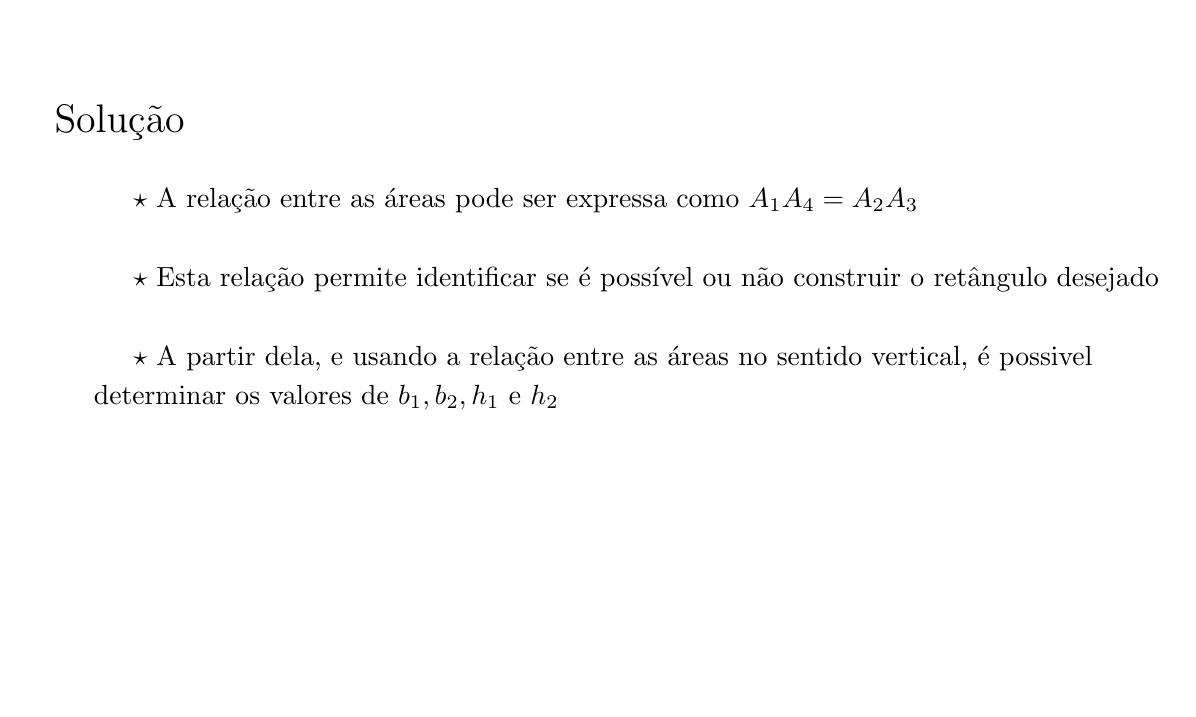
\begin{tikzpicture}
\node[draw,opacity=0] at (0, 0) {x};
\node[draw,opacity=0] at (14, 8) {x};

	\node[anchor=west] (title) at (0.0, 7.0) { \Large \bbbold{Solução} };

	\node[anchor=west] (a) at (1.0, 6.0) { $\star$ \bbtext{A relação entre as áreas pode ser expressa como $A_1A_4 = A_2A_3$} };


	\node[anchor=west] (b) at (1.0, 5.0) { $\star$ \bbtext{Esta relação permite identificar se é possível ou não construir o retângulo desejado} };

	\node[anchor=west] (c) at (1.0, 4.0) { $\star$ \bbtext{A partir dela, e usando a relação entre as áreas no sentido vertical, é possivel} };

	\node[anchor=west] (c1) at (0.5, 3.5) { \bbtext{determinar os valores de $b_1, b_2, h_1$ e $h_2$} };

\end{tikzpicture}
\end{frame}
\begin{frame}[plain,t]
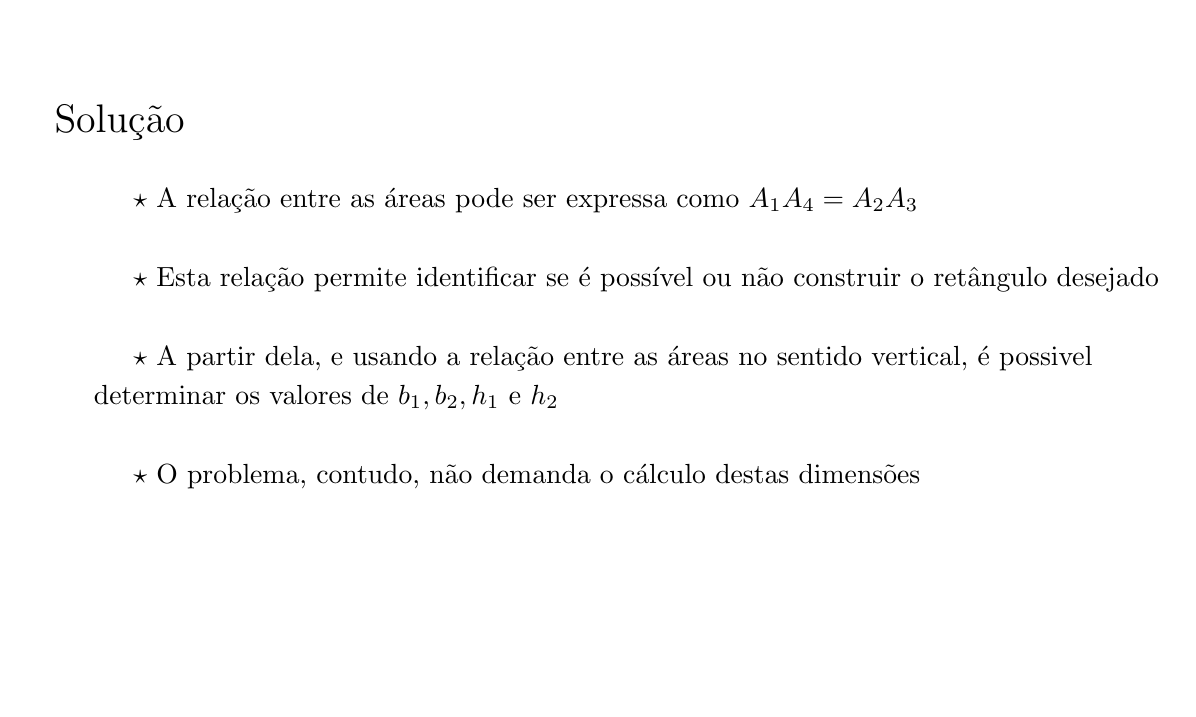
\begin{tikzpicture}
\node[draw,opacity=0] at (0, 0) {x};
\node[draw,opacity=0] at (14, 8) {x};

	\node[anchor=west] (title) at (0.0, 7.0) { \Large \bbbold{Solução} };

	\node[anchor=west] (a) at (1.0, 6.0) { $\star$ \bbtext{A relação entre as áreas pode ser expressa como $A_1A_4 = A_2A_3$} };


	\node[anchor=west] (b) at (1.0, 5.0) { $\star$ \bbtext{Esta relação permite identificar se é possível ou não construir o retângulo desejado} };

	\node[anchor=west] (c) at (1.0, 4.0) { $\star$ \bbtext{A partir dela, e usando a relação entre as áreas no sentido vertical, é possivel} };

	\node[anchor=west] (c1) at (0.5, 3.5) { \bbtext{determinar os valores de $b_1, b_2, h_1$ e $h_2$} };

	\node[anchor=west] (d) at (1.0, 2.5) { $\star$ \bbtext{O problema, contudo, não demanda o cálculo destas dimensões} };

\end{tikzpicture}
\end{frame}
\begin{frame}[plain,t]
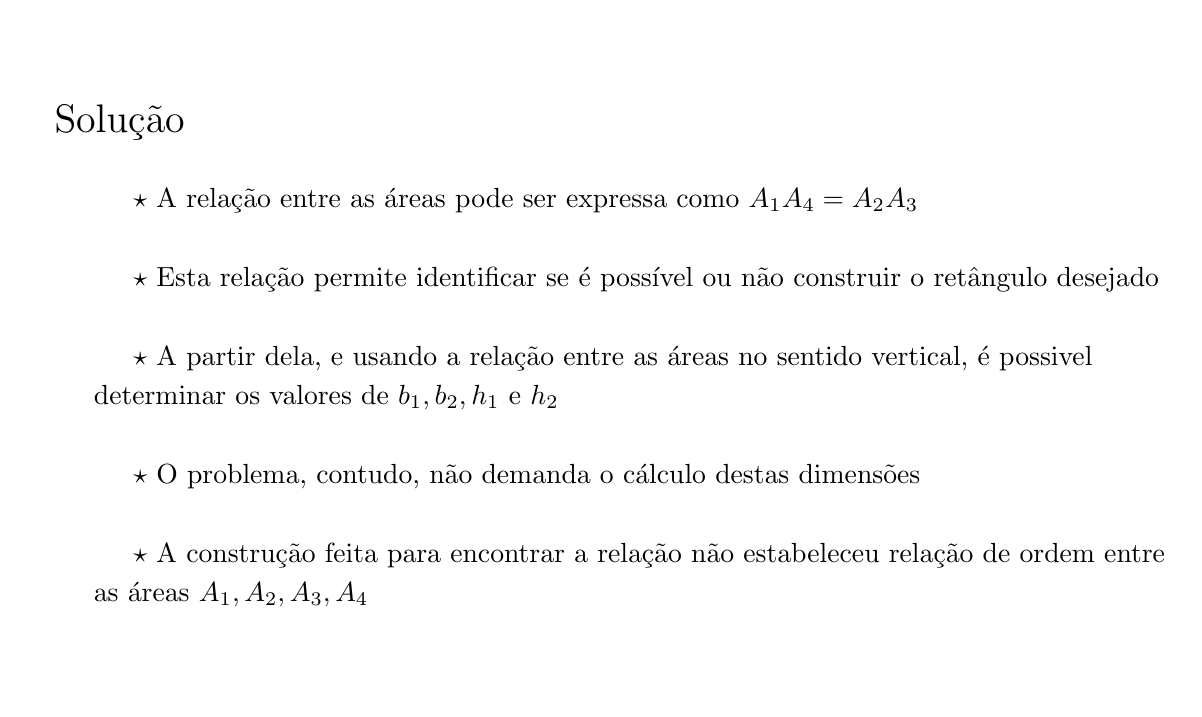
\begin{tikzpicture}
\node[draw,opacity=0] at (0, 0) {x};
\node[draw,opacity=0] at (14, 8) {x};

	\node[anchor=west] (title) at (0.0, 7.0) { \Large \bbbold{Solução} };

	\node[anchor=west] (a) at (1.0, 6.0) { $\star$ \bbtext{A relação entre as áreas pode ser expressa como $A_1A_4 = A_2A_3$} };


	\node[anchor=west] (b) at (1.0, 5.0) { $\star$ \bbtext{Esta relação permite identificar se é possível ou não construir o retângulo desejado} };

	\node[anchor=west] (c) at (1.0, 4.0) { $\star$ \bbtext{A partir dela, e usando a relação entre as áreas no sentido vertical, é possivel} };

	\node[anchor=west] (c1) at (0.5, 3.5) { \bbtext{determinar os valores de $b_1, b_2, h_1$ e $h_2$} };

	\node[anchor=west] (d) at (1.0, 2.5) { $\star$ \bbtext{O problema, contudo, não demanda o cálculo destas dimensões} };

	\node[anchor=west] (e) at (1.0, 1.5) { $\star$ \bbtext{A construção feita para encontrar a relação não estabeleceu relação de ordem entre} };

	\node[anchor=west] (e1) at (0.5, 1.0) { \bbtext{as áreas $A_1, A_2, A_3, A_4$} };

\end{tikzpicture}
\end{frame}
\begin{frame}[plain,t]
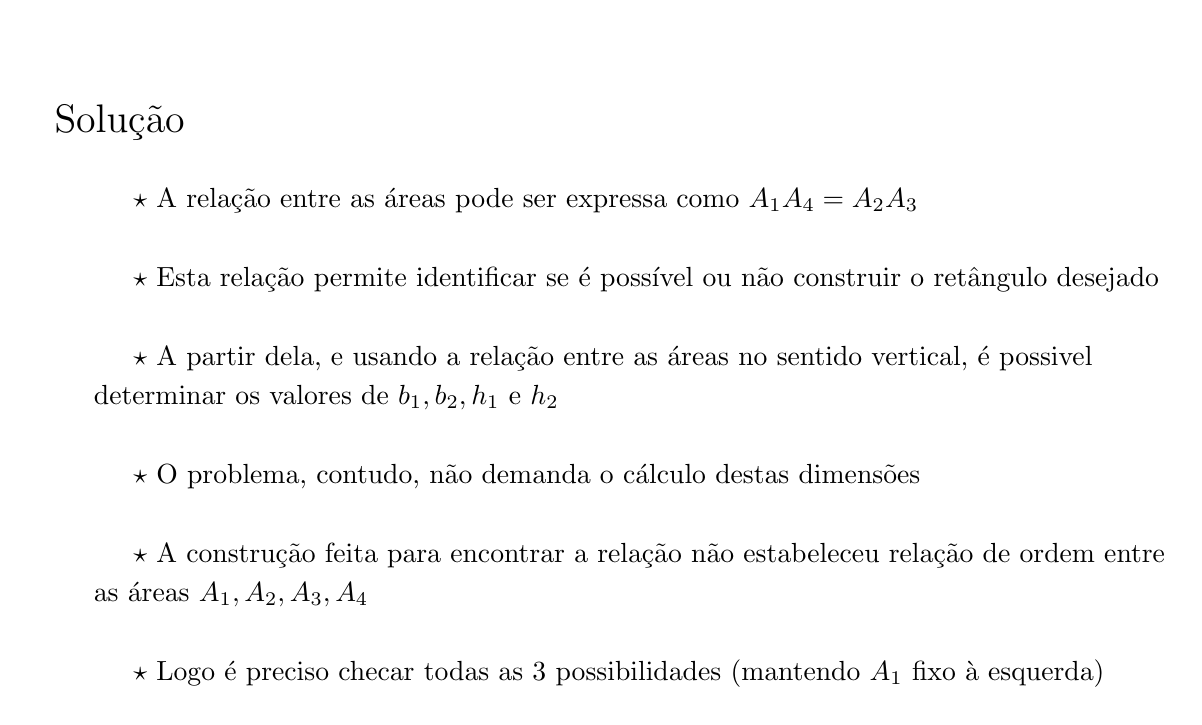
\begin{tikzpicture}
\node[draw,opacity=0] at (0, 0) {x};
\node[draw,opacity=0] at (14, 8) {x};

	\node[anchor=west] (title) at (0.0, 7.0) { \Large \bbbold{Solução} };

	\node[anchor=west] (a) at (1.0, 6.0) { $\star$ \bbtext{A relação entre as áreas pode ser expressa como $A_1A_4 = A_2A_3$} };


	\node[anchor=west] (b) at (1.0, 5.0) { $\star$ \bbtext{Esta relação permite identificar se é possível ou não construir o retângulo desejado} };

	\node[anchor=west] (c) at (1.0, 4.0) { $\star$ \bbtext{A partir dela, e usando a relação entre as áreas no sentido vertical, é possivel} };

	\node[anchor=west] (c1) at (0.5, 3.5) { \bbtext{determinar os valores de $b_1, b_2, h_1$ e $h_2$} };

	\node[anchor=west] (d) at (1.0, 2.5) { $\star$ \bbtext{O problema, contudo, não demanda o cálculo destas dimensões} };

	\node[anchor=west] (e) at (1.0, 1.5) { $\star$ \bbtext{A construção feita para encontrar a relação não estabeleceu relação de ordem entre} };

	\node[anchor=west] (e1) at (0.5, 1.0) { \bbtext{as áreas $A_1, A_2, A_3, A_4$} };


	\node[anchor=west] (f) at (1.0, 0.0) { $\star$ \bbtext{Logo é preciso checar todas as 3 possibilidades (mantendo $A_1$ fixo à esquerda)} };

\end{tikzpicture}
\end{frame}
\begin{frame}[plain,t]
\begin{tikzpicture}
\node[draw,opacity=0] at (0, 0) {x};
\node[draw,opacity=0] at (14, 8) {x};

	\node[anchor=west] (title) at (0.0, 7.0) { \Large \bbbold{Solução $O(1)$ em C++} };

\end{tikzpicture}
\end{frame}
\begin{frame}[plain,t]
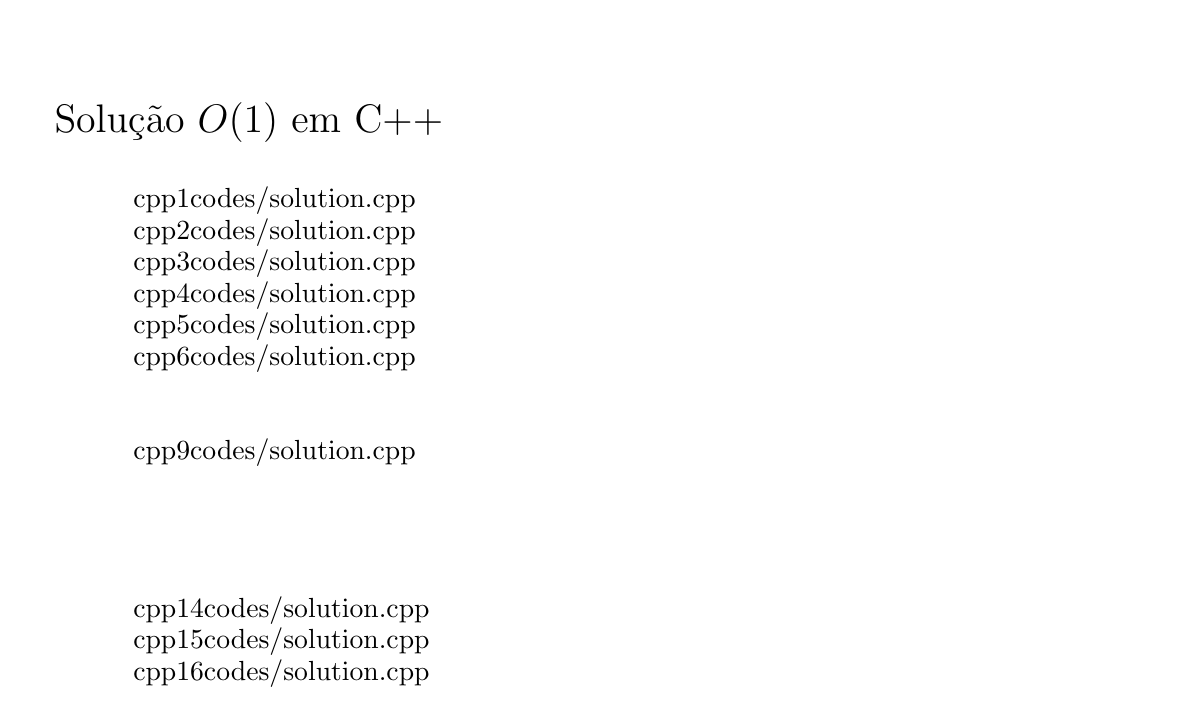
\begin{tikzpicture}
\node[draw,opacity=0] at (0, 0) {x};
\node[draw,opacity=0] at (14, 8) {x};

	\node[anchor=west] (title) at (0.0, 7.0) { \Large \bbbold{Solução $O(1)$ em C++} };


	\node[anchor=west] (line1) at (1.0, 6.0) { \inputline{cpp}{1}{codes/solution.cpp} };

	\node[anchor=west] (line2) at (1.0, 5.6) { \inputline{cpp}{2}{codes/solution.cpp} };

	\node[anchor=west] (line3) at (1.0, 5.2) { \inputline{cpp}{3}{codes/solution.cpp} };

	\node[anchor=west] (line4) at (1.0, 4.8) { \inputline{cpp}{4}{codes/solution.cpp} };

	\node[anchor=west] (line5) at (1.0, 4.4) { \inputline{cpp}{5}{codes/solution.cpp} };

	\node[anchor=west] (line6) at (1.0, 4.0) { \inputline{cpp}{6}{codes/solution.cpp} };



	\node[anchor=west] (line9) at (1.0, 2.8) { \inputline{cpp}{9}{codes/solution.cpp} };





	\node[anchor=west] (line14) at (1.0, 0.8) { \inputline{cpp}{14}{codes/solution.cpp} };

	\node[anchor=west] (line15) at (1.0, 0.4) { \inputline{cpp}{15}{codes/solution.cpp} };

	\node[anchor=west] (line16) at (1.0, -0.0) { \inputline{cpp}{16}{codes/solution.cpp} };


\end{tikzpicture}
\end{frame}
\begin{frame}[plain,t]
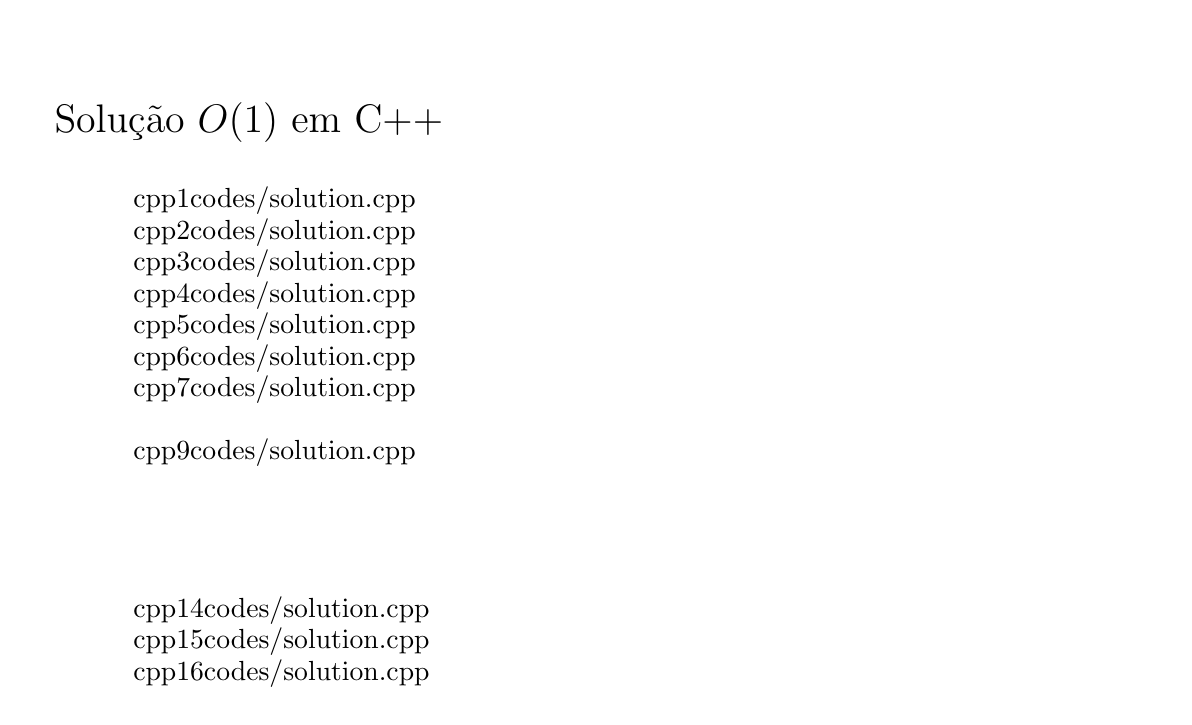
\begin{tikzpicture}
\node[draw,opacity=0] at (0, 0) {x};
\node[draw,opacity=0] at (14, 8) {x};

	\node[anchor=west] (title) at (0.0, 7.0) { \Large \bbbold{Solução $O(1)$ em C++} };


	\node[anchor=west] (line1) at (1.0, 6.0) { \inputline{cpp}{1}{codes/solution.cpp} };

	\node[anchor=west] (line2) at (1.0, 5.6) { \inputline{cpp}{2}{codes/solution.cpp} };

	\node[anchor=west] (line3) at (1.0, 5.2) { \inputline{cpp}{3}{codes/solution.cpp} };

	\node[anchor=west] (line4) at (1.0, 4.8) { \inputline{cpp}{4}{codes/solution.cpp} };

	\node[anchor=west] (line5) at (1.0, 4.4) { \inputline{cpp}{5}{codes/solution.cpp} };

	\node[anchor=west] (line6) at (1.0, 4.0) { \inputline{cpp}{6}{codes/solution.cpp} };

	\node[anchor=west] (line7) at (1.0, 3.6) { \inputline{cpp}{7}{codes/solution.cpp} };


	\node[anchor=west] (line9) at (1.0, 2.8) { \inputline{cpp}{9}{codes/solution.cpp} };





	\node[anchor=west] (line14) at (1.0, 0.8) { \inputline{cpp}{14}{codes/solution.cpp} };

	\node[anchor=west] (line15) at (1.0, 0.4) { \inputline{cpp}{15}{codes/solution.cpp} };

	\node[anchor=west] (line16) at (1.0, -0.0) { \inputline{cpp}{16}{codes/solution.cpp} };



\end{tikzpicture}
\end{frame}
\begin{frame}[plain,t]
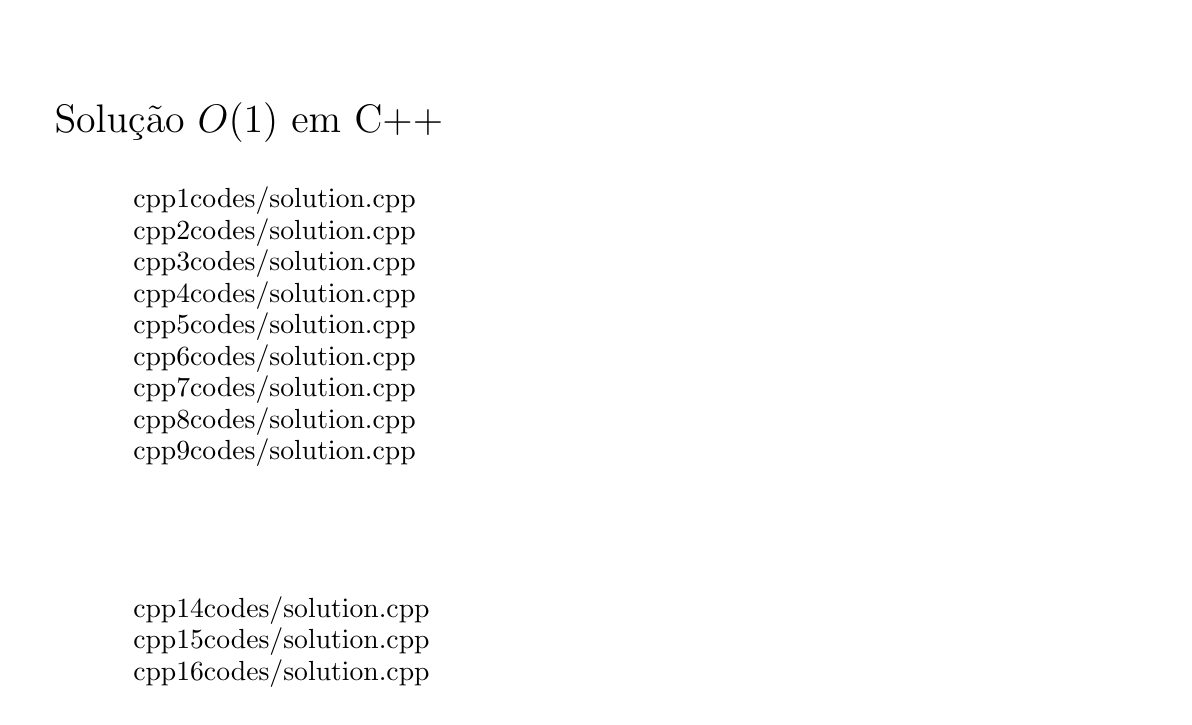
\begin{tikzpicture}
\node[draw,opacity=0] at (0, 0) {x};
\node[draw,opacity=0] at (14, 8) {x};

	\node[anchor=west] (title) at (0.0, 7.0) { \Large \bbbold{Solução $O(1)$ em C++} };


	\node[anchor=west] (line1) at (1.0, 6.0) { \inputline{cpp}{1}{codes/solution.cpp} };

	\node[anchor=west] (line2) at (1.0, 5.6) { \inputline{cpp}{2}{codes/solution.cpp} };

	\node[anchor=west] (line3) at (1.0, 5.2) { \inputline{cpp}{3}{codes/solution.cpp} };

	\node[anchor=west] (line4) at (1.0, 4.8) { \inputline{cpp}{4}{codes/solution.cpp} };

	\node[anchor=west] (line5) at (1.0, 4.4) { \inputline{cpp}{5}{codes/solution.cpp} };

	\node[anchor=west] (line6) at (1.0, 4.0) { \inputline{cpp}{6}{codes/solution.cpp} };

	\node[anchor=west] (line7) at (1.0, 3.6) { \inputline{cpp}{7}{codes/solution.cpp} };

	\node[anchor=west] (line8) at (1.0, 3.2) { \inputline{cpp}{8}{codes/solution.cpp} };

	\node[anchor=west] (line9) at (1.0, 2.8) { \inputline{cpp}{9}{codes/solution.cpp} };





	\node[anchor=west] (line14) at (1.0, 0.8) { \inputline{cpp}{14}{codes/solution.cpp} };

	\node[anchor=west] (line15) at (1.0, 0.4) { \inputline{cpp}{15}{codes/solution.cpp} };

	\node[anchor=west] (line16) at (1.0, -0.0) { \inputline{cpp}{16}{codes/solution.cpp} };




\end{tikzpicture}
\end{frame}
\begin{frame}[plain,t]
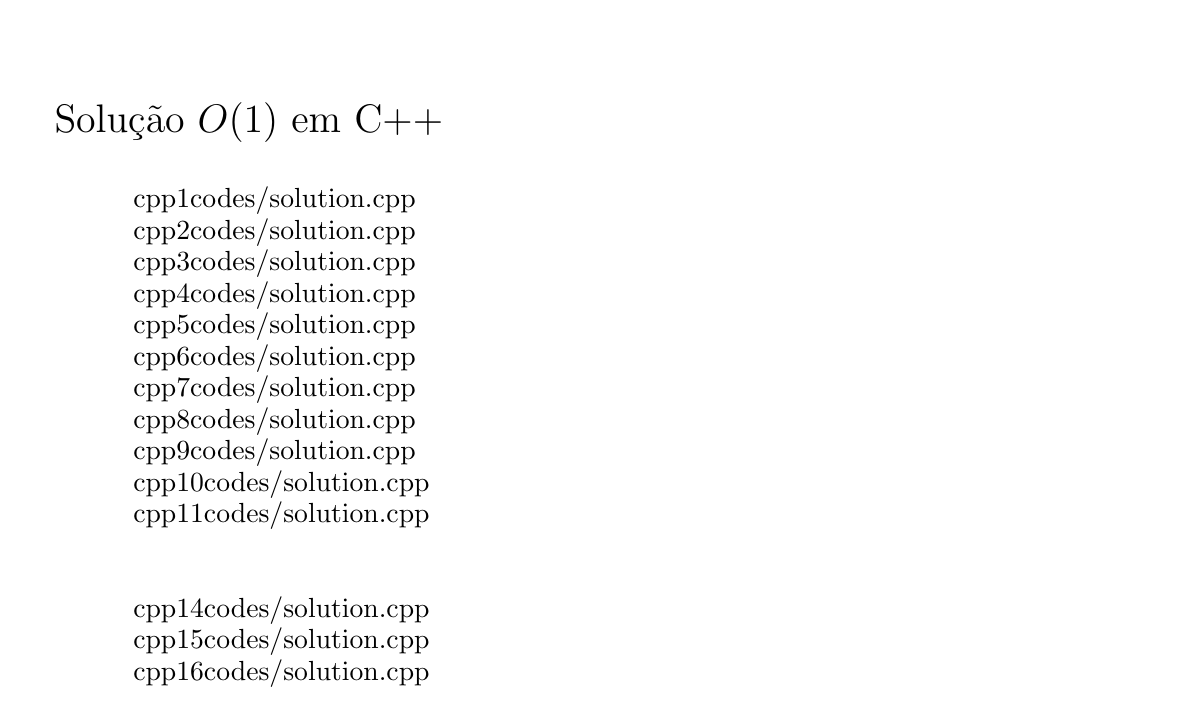
\begin{tikzpicture}
\node[draw,opacity=0] at (0, 0) {x};
\node[draw,opacity=0] at (14, 8) {x};

	\node[anchor=west] (title) at (0.0, 7.0) { \Large \bbbold{Solução $O(1)$ em C++} };


	\node[anchor=west] (line1) at (1.0, 6.0) { \inputline{cpp}{1}{codes/solution.cpp} };

	\node[anchor=west] (line2) at (1.0, 5.6) { \inputline{cpp}{2}{codes/solution.cpp} };

	\node[anchor=west] (line3) at (1.0, 5.2) { \inputline{cpp}{3}{codes/solution.cpp} };

	\node[anchor=west] (line4) at (1.0, 4.8) { \inputline{cpp}{4}{codes/solution.cpp} };

	\node[anchor=west] (line5) at (1.0, 4.4) { \inputline{cpp}{5}{codes/solution.cpp} };

	\node[anchor=west] (line6) at (1.0, 4.0) { \inputline{cpp}{6}{codes/solution.cpp} };

	\node[anchor=west] (line7) at (1.0, 3.6) { \inputline{cpp}{7}{codes/solution.cpp} };

	\node[anchor=west] (line8) at (1.0, 3.2) { \inputline{cpp}{8}{codes/solution.cpp} };

	\node[anchor=west] (line9) at (1.0, 2.8) { \inputline{cpp}{9}{codes/solution.cpp} };

	\node[anchor=west] (line10) at (1.0, 2.4) { \inputline{cpp}{10}{codes/solution.cpp} };

	\node[anchor=west] (line11) at (1.0, 2.0) { \inputline{cpp}{11}{codes/solution.cpp} };



	\node[anchor=west] (line14) at (1.0, 0.8) { \inputline{cpp}{14}{codes/solution.cpp} };

	\node[anchor=west] (line15) at (1.0, 0.4) { \inputline{cpp}{15}{codes/solution.cpp} };

	\node[anchor=west] (line16) at (1.0, -0.0) { \inputline{cpp}{16}{codes/solution.cpp} };





\end{tikzpicture}
\end{frame}
\begin{frame}[plain,t]
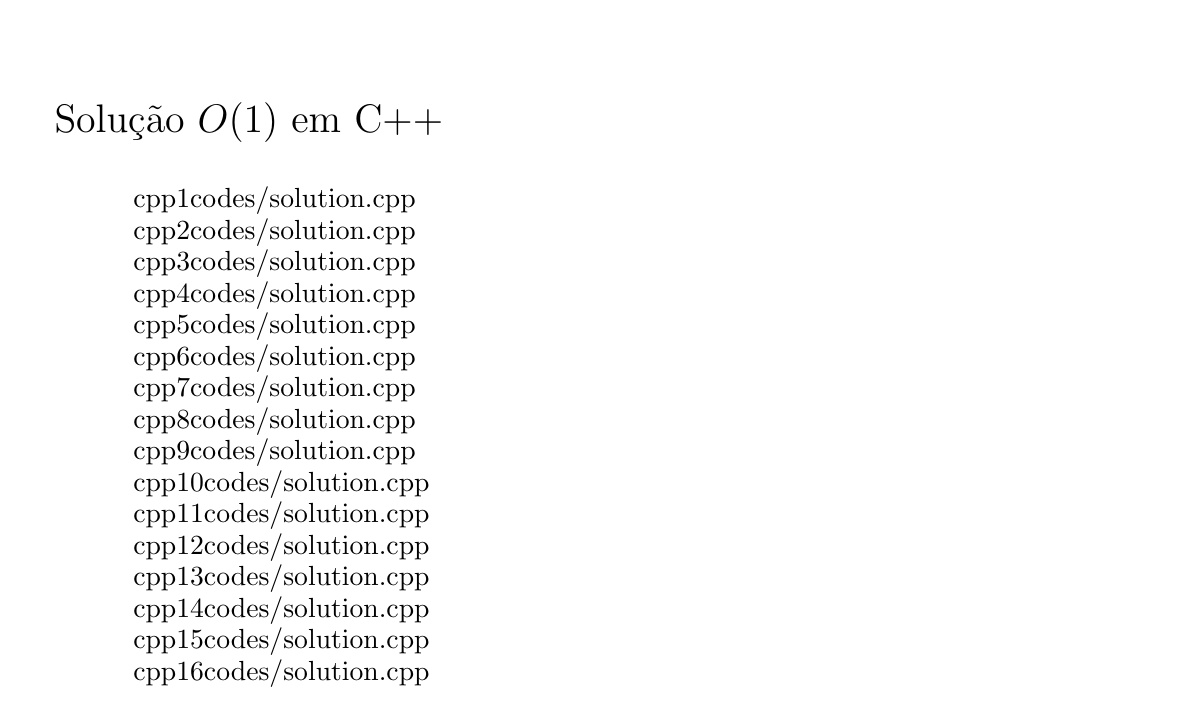
\begin{tikzpicture}
\node[draw,opacity=0] at (0, 0) {x};
\node[draw,opacity=0] at (14, 8) {x};

	\node[anchor=west] (title) at (0.0, 7.0) { \Large \bbbold{Solução $O(1)$ em C++} };


	\node[anchor=west] (line1) at (1.0, 6.0) { \inputline{cpp}{1}{codes/solution.cpp} };

	\node[anchor=west] (line2) at (1.0, 5.6) { \inputline{cpp}{2}{codes/solution.cpp} };

	\node[anchor=west] (line3) at (1.0, 5.2) { \inputline{cpp}{3}{codes/solution.cpp} };

	\node[anchor=west] (line4) at (1.0, 4.8) { \inputline{cpp}{4}{codes/solution.cpp} };

	\node[anchor=west] (line5) at (1.0, 4.4) { \inputline{cpp}{5}{codes/solution.cpp} };

	\node[anchor=west] (line6) at (1.0, 4.0) { \inputline{cpp}{6}{codes/solution.cpp} };

	\node[anchor=west] (line7) at (1.0, 3.6) { \inputline{cpp}{7}{codes/solution.cpp} };

	\node[anchor=west] (line8) at (1.0, 3.2) { \inputline{cpp}{8}{codes/solution.cpp} };

	\node[anchor=west] (line9) at (1.0, 2.8) { \inputline{cpp}{9}{codes/solution.cpp} };

	\node[anchor=west] (line10) at (1.0, 2.4) { \inputline{cpp}{10}{codes/solution.cpp} };

	\node[anchor=west] (line11) at (1.0, 2.0) { \inputline{cpp}{11}{codes/solution.cpp} };

	\node[anchor=west] (line12) at (1.0, 1.6) { \inputline{cpp}{12}{codes/solution.cpp} };

	\node[anchor=west] (line13) at (1.0, 1.2) { \inputline{cpp}{13}{codes/solution.cpp} };

	\node[anchor=west] (line14) at (1.0, 0.8) { \inputline{cpp}{14}{codes/solution.cpp} };

	\node[anchor=west] (line15) at (1.0, 0.4) { \inputline{cpp}{15}{codes/solution.cpp} };

	\node[anchor=west] (line16) at (1.0, -0.0) { \inputline{cpp}{16}{codes/solution.cpp} };






\end{tikzpicture}
\end{frame}
\end{document}
